% =====================================================================
%  Chapitre 5 -- CNN au-dela de la classification
%  Partie b : CNN 1D pour les series temporelles, autres modalites,
%             quiz, a retenir, TP5
% =====================================================================

\begin{frame}{Les CNN pour les séries temporelles}
\begin{columns}[t]
\begin{column}{0.50\textwidth}
\begin{itemize}
  \item Une \textbf{série temporelle} est un signal : une valeur mesurée
  à chaque instant.
  \item Exemples : électrocardiogramme (ECG), trafic routier heure par heure,
  météo, vibrations d'une machine, cours d'une action.
  \item Le motif d'intérêt (un battement, un pic de trafic) peut apparaître
  \emph{n'importe où} dans le temps.
  \item Un CNN 1D réutilise exactement les idées vues en 2D :
  \textbf{localité} dans le temps et \textbf{partage des poids} le long du signal.
\end{itemize}
\end{column}
\begin{column}{0.48\textwidth}
\begin{kbox}[La transposition]
L'axe des temps joue le rôle des axes d'une image. Un noyau de longueur
$k$ glisse le long du signal ; la même réponse est reconnue partout,
quelle que soit sa position temporelle.
\end{kbox}

\end{column}
\end{columns}
% [fix] bloc deplace
\end{frame}
\begin{frame}{Les CNN pour les séries temporelles (suite)}
\begin{ebox}[Un même mot, deux dimensions]
Image $=$ deux axes (espace). Série temporelle $=$ un axe (temps). Le
principe convolutif est identique ; seul le nombre d'axes change.
\end{ebox}
\end{frame}

\begin{frame}{Un noyau 1D remplace un noyau 2D}
\begin{columns}[t]
\begin{column}{0.52\textwidth}
\begin{itemize}
  \item Un noyau 2D est une petite matrice ($3 \times 3$, $5 \times 5$).
  \item Un noyau 1D est un petit \textbf{vecteur}, de longueur $k$
  (souvent 3, 5, 7, 9).
  \item La sortie, en position $t$, est une somme pondérée :
\end{itemize}
\[
y[t]=\sum_{j=0}^{k-1} x[t+j]\,w[j] + b
\]
\begin{itemize}
  \item Le noyau \emph{glisse} d'un pas le long du temps ; un nombre réduit
  de poids suffit pour tout le signal.
\end{itemize}
\end{column}
\begin{column}{0.46\textwidth}
\begin{kbox}[Correspondance directe]
2D : hauteur $\times$ largeur, noyau $(k_h, k_w)$.\newline
1D : longueur, noyau $(k,)$.\newline
Pooling, ReLU, padding, stride : idem, sur un seul axe.
\end{kbox}

\end{column}
\end{columns}
% [fix] bloc deplace
\end{frame}
\begin{frame}{Un noyau 1D remplace un noyau 2D (suite)}
\begin{wbox}[Une image $1 \times N$ n'est pas un signal]
Une image de hauteur 1 n'a de sens spatial que sur un axe ; le CNN 1D traite
cet axe comme un \emph{temps}, pas comme une dimension d'image.
\end{wbox}
\end{frame}

\begin{frame}[fragile]{La forme des tenseurs en 1D}
\begin{columns}[t]
\begin{column}{0.50\textwidth}
\begin{itemize}
  \item En 2D, un tenseur d'activation a la forme
  \py{(lot, canaux, hauteur, largeur)}.
  \item En 1D, il a la forme \py{(lot, canaux, longueur)}.
  \item Un \emph{canal} 1D est un signal d'une source : par exemple les
  dérivations d'un ECG, ou plusieurs capteurs d'une machine.
  \item Le \py{Flatten} avant les couches denses suit le même rôle : mettre à
  plat canaux et temps.
\end{itemize}
\end{column}
\begin{column}{0.48\textwidth}
\begin{codebox}[Forme des tenseurs (PyTorch)]
\begin{lstlisting}
import torch
# image : (lot, canaux, H, W)
x2 = torch.randn(8, 3, 32, 32)
# signal : (lot, canaux, longueur)
x1 = torch.randn(8, 3, 1200)
conv1d = torch.nn.Conv1d(3, 16, kernel_size=5)
print(conv1d(x1).shape)
# -> torch.Size([8, 16, 1196])
\end{lstlisting}
\end{codebox}
\end{column}
\end{columns}
\end{frame}

\begin{frame}{Étude de cas : détecter les battements d'un ECG}
\begin{columns}[t]
\begin{column}{0.52\textwidth}
\centering
\end{column}
\begin{column}{0.45\textwidth}
\begin{itemize}
  \item Signal étudié : un ECG à \textbf{72 battements par minute},
  d'une durée de \textbf{10 s}, échantillonné en \textbf{1\,200 points}.
  \item Cette cadence correspond à environ un battement toutes les
  $0{,}83$ s.
  \item Le motif à détecter est le \textbf{complexe QRS} : la pointe
  caractéristique de chaque battement.
  \item Une analyse par filtre 1D et seuil détecte \textbf{11 battements}
  sur ces 10 s.
\end{itemize}
\end{column}
\end{columns}
\vspace{0.5mm}
\begin{kbox}[Le problème posé]
Détecter \emph{où} se trouvent les battements, sans les compter à l'\oe{}il :
c'est une tâche de \textbf{détection de motif} sur un signal 1D.
\end{kbox}
% [fix] figure sortie
\end{frame}

\begin{frame}{Étude de cas : détecter les battements d'un ECG --- la figure}\begin{center}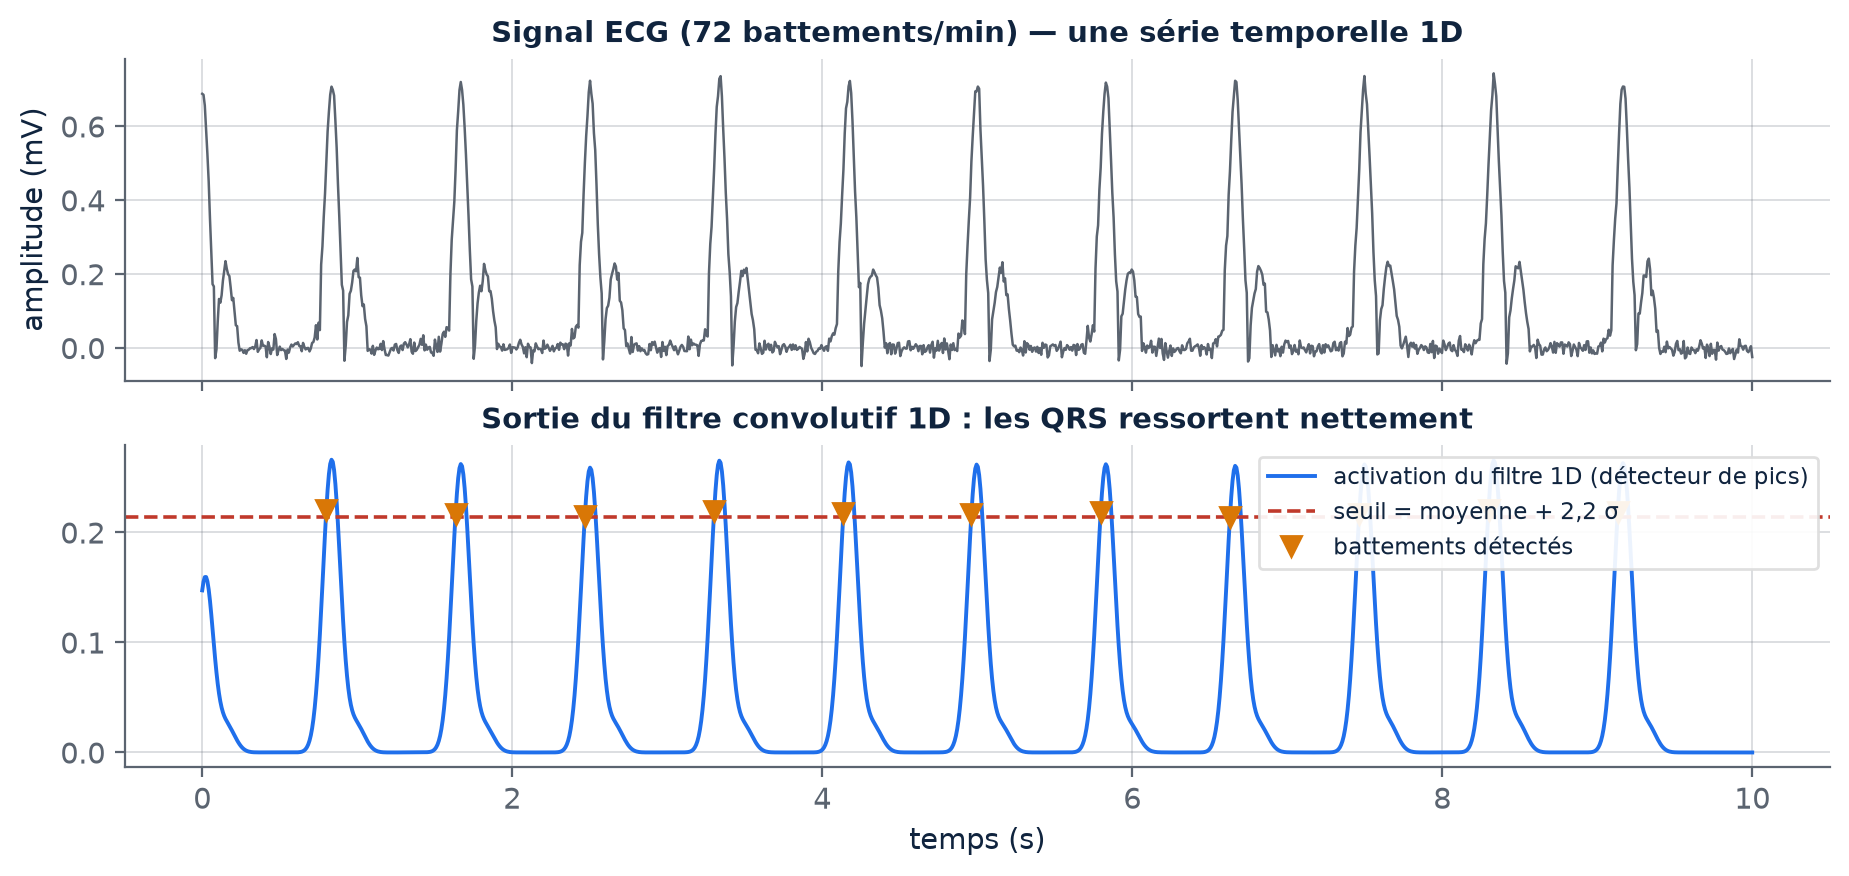
\includegraphics[width=.92\textwidth]{j05_cnn1d_ecg.png}\end{center}\end{frame}

\begin{frame}{Le filtre 1D et le seuil statistique}
\begin{columns}[t]
\begin{column}{0.50\textwidth}
\begin{itemize}
  \item Étape 1 : un \textbf{filtre 1D} met en évidence les fronts raides
  (le pas de QRS), par exemple un noyau différenciateur.
  \item Étape 2 : on calcule la \textbf{moyenne} et l'écart-type de l'énergie
  du signal filtré.
  \item Étape 3 : on déclare « battement » toute position où l'énergie dépasse
  \[ \text{moyenne} + 2{,}2\,\sigma \]
  \item $\sigma$ : écart-type de l'énergie du signal filtré.
\end{itemize}
\end{column}
\begin{column}{0.48\textwidth}
\begin{kbox}[Le seuil retenu]
Le seuil de détection des QRS vaut \textbf{moyenne $+\,2{,}2$ sigma}. Un seuil
trop bas capte le bruit ; un seuil trop haut manque des battements.
\end{kbox}
\begin{ebox}[Une méthode classique]
Filtrer, calculer une énergie, appliquer un seuil, puis regrouper les
détections proches : c'est exactement la logique d'une chaîne de prétraitement
historique, que le CNN 1D peut \emph{apprendre} au lieu de la coder à la main.
\end{ebox}
\end{column}
\end{columns}
\end{frame}

\begin{frame}[fragile]{Détection des QRS en Python}
\begin{columns}[t]
\begin{column}{0.52\textwidth}
\begin{codebox}[Filtre 1D + seuil moyenne + 2,2 sigma]
\begin{lstlisting}
import numpy as np
from scipy.signal import convolve

# signal : 1200 points, ECG a 72 bpm
filtre = np.array([-1, -2, 0, 2, 1])   # differenciateur 1D
energie = np.abs(convolve(x, filtre, mode='same'))

mu = energie.mean()
sigma = energie.std()
seuil = mu + 2.2 * sigma          # seuil retenu

detections = energie > seuil
print(detections.sum())           # 11 battements
\end{lstlisting}
\end{codebox}
\end{column}
\begin{column}{0.46\textwidth}
\begin{itemize}
  \item Le noyau 1D \py{[-1, -2, 0, 2, 1]} amplifie les fronts montants
  et descendants.
  \item Le seuil \py{mu + 2.2 * sigma} s'adapte automatiquement à
  l'amplitude du signal.
  \item En pratique on regroupe ensuite les détections contiguës en
  \emph{un} battement (une localisation par QRS).
\end{itemize}
\begin{wbox}[Variabilité]
Le seuil dépend de la qualité du signal : sur un ECG bruité, il faut
d'abord filtrer les basses fréquences.
\end{wbox}
\end{column}
\end{columns}
\end{frame}

\begin{frame}{Étude de cas : le trafic routier}
\begin{columns}[t]
\begin{column}{0.52\textwidth}
\centering
\end{column}
\begin{column}{0.45\textwidth}
\begin{itemize}
  \item Un compteur routier relève, heure après heure, le nombre de véhicules.
  \item Deux rythmes se superposent :
  \begin{itemize}
    \item un \textbf{cycle journalier} de \textbf{24 h} (pics du matin
    et du soir, creux nocturne) ;
    \item un \textbf{cycle hebdomadaire} (jours ouvrés et week-end).
  \end{itemize}
  \item Le graphique porte sur un horizon de \textbf{4 jours}.
\end{itemize}
\end{column}
\end{columns}
\vspace{0.5mm}
\begin{kbox}[Ce que la convolution apporte]
Un noyau de longueur proche de la période d'un cycle apprend à repérer ce motif
périodique, quelle que soit sa position dans la série : c'est la
\emph{localité} transposée au temps.
\end{kbox}
% [fix] figure sortie
\end{frame}

\begin{frame}{Étude de cas : le trafic routier --- la figure}\begin{center}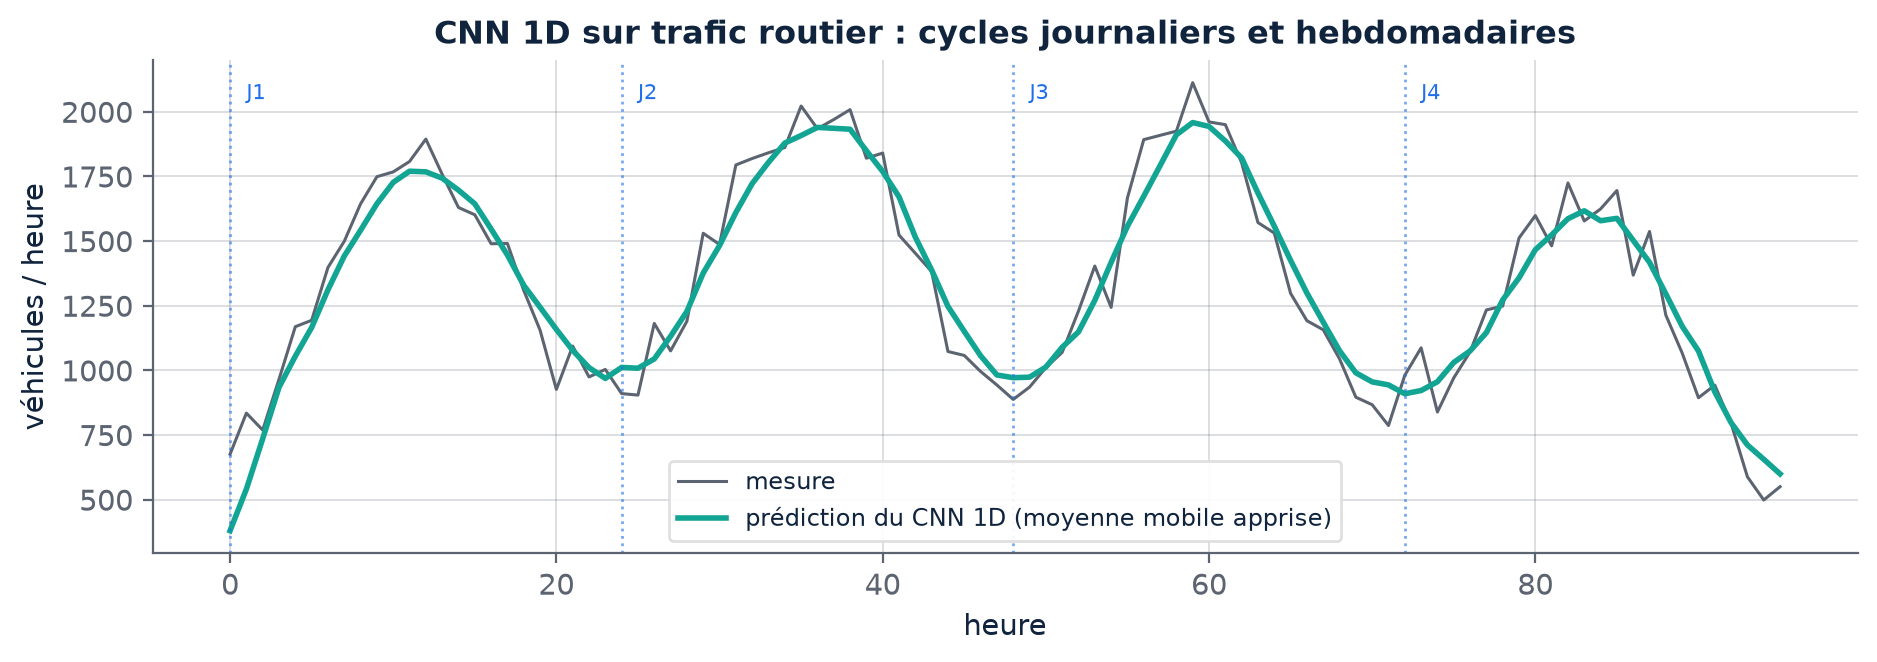
\includegraphics[width=.92\textwidth]{j06_cnn1d_trafic.png}\end{center}\end{frame}

\begin{frame}{Autres modalités : même principe, autres axes}
\begin{columns}[t]
\begin{column}{0.50\textwidth}
\centering
\end{column}
\begin{column}{0.48\textwidth}
\begin{itemize}
  \item \textbf{Audio} : on convertit le son en \textbf{spectrogramme}, une
  image temps $\times$ fréquences ; le CNN 2D s'applique tel quel.
  \item \textbf{Texte} : une séquence de mots ou de caractères se traite
  comme un signal 1D (noyaux sur les mots voisins).
  \item \textbf{Imagerie 3D} : un scan médical est un volume ; le noyau
  devient un petit cube ($3 \times 3 \times 3$).
\end{itemize}
\end{column}
\end{columns}
\vspace{0.5mm}
\begin{wbox}[Choisir la dimension du noyau]
Le noyau se choisit selon la \emph{structure} des données : 1D pour une
séquence, 2D pour une image, 3D pour un volume. Le réseau reste le même outil.
\end{wbox}
% [fix] figure sortie
\end{frame}

\begin{frame}{Autres modalités : même principe, autres axes --- la figure}\begin{center}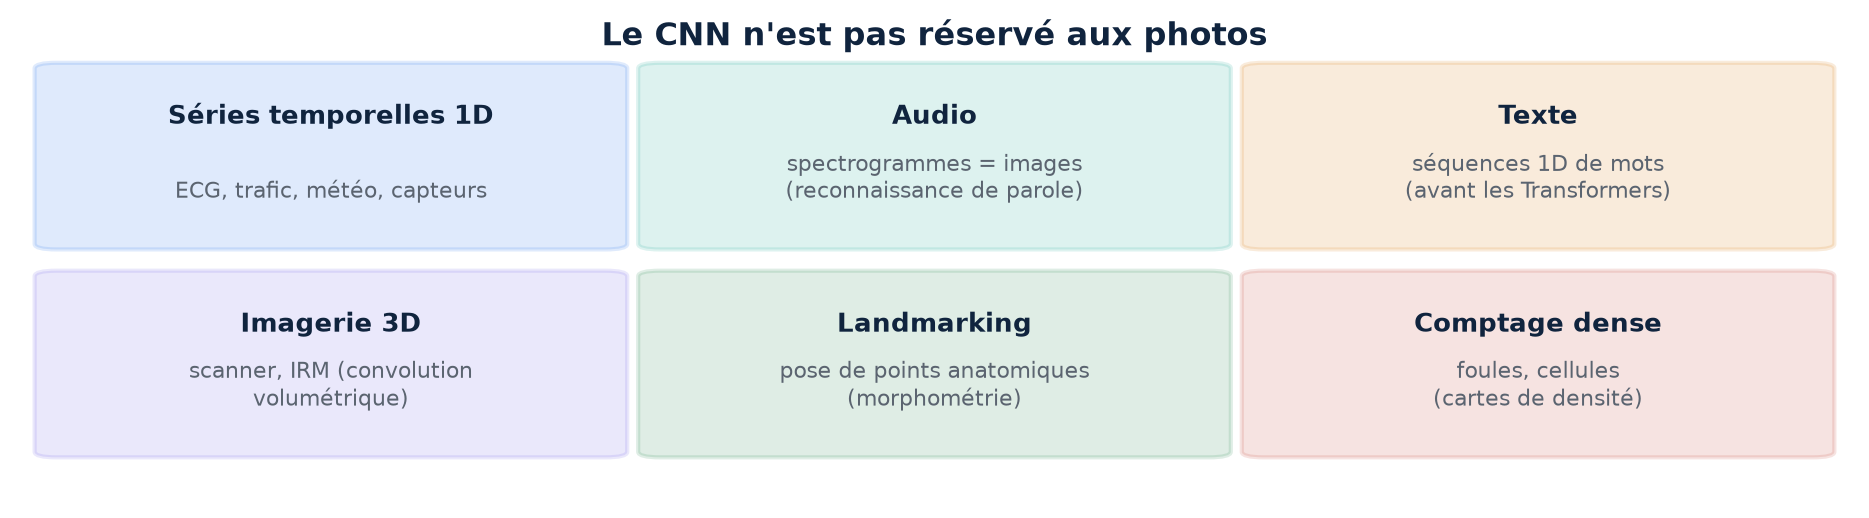
\includegraphics[width=.92\textwidth]{j07_autres_modalites.png}\end{center}\end{frame}

\begin{frame}{Landmarking et comptage dense}
\begin{columns}[t]
\begin{column}{0.48\textwidth}
\begin{ebox}[Landmarking (points anatomiques)]
Le CNN prédit les coordonnées de points précis sur une image
(coins des yeux, articulations, points de morphométrie). On passe d'une
classification à une \textbf{régression}.
\end{ebox}
\begin{kbox}[Comptage dense (\emph{crowd counting})]
Le réseau produit une \emph{carte de densité} : la somme des valeurs de la
carte donne le nombre estimé d'objets, sans boîte individuelle.
\end{kbox}
\end{column}
\begin{column}{0.48\textwidth}
\begin{itemize}
  \item Ces tâches montrent la \textbf{souplesse de la tête de sortie} :
  - classification : un vecteur de probabilités ;
  - détection : des boîtes et des scores ;
  - segmentation : un masque dense ;
  - landmarking : des coordonnées continues ;
  - comptage dense : une carte de densité.
  \item Le cœur convolutif (encodeur) peut être \textbf{partagé} entre ces
  tâches.
\end{itemize}
\end{column}
\end{columns}
\end{frame}

\begin{frame}{Quiz}
\begin{columns}[t]
\begin{column}{0.49\textwidth}
\begin{qbox}[Question 1]
Quelle est la différence entre la \emph{classification} et la
\emph{détection} d'objets ?
\begin{itemize}
  \item[(a)] Aucune, ce sont deux noms de la même tâche
  \item[(b)] La détection localise \emph{et} classifie (boîtes englobantes)
  \item[(c)] La détection ne classe pas les objets
\end{itemize}
\end{qbox}
\begin{qbox}[Question 2]
Que mesure l'IoU entre deux boîtes englobantes ?
\begin{itemize}
  \item[(a)] La vitesse du détecteur
  \item[(b)] Le recouvrement : surface de l'intersection sur celle de l'union
  \item[(c)] Le nombre de classes présentes
\end{itemize}
\end{qbox}
\end{column}
\begin{column}{0.49\textwidth}
\begin{qbox}[Question 3]
À quoi sert la suppression des non-maxima (NMS) ?
\begin{itemize}
  \item[(a)] À accélérer l'entraînement
  \item[(b)] À supprimer les boîtes en double pour un même objet
  \item[(c)] À augmenter la résolution de l'image
\end{itemize}
\end{qbox}
\begin{qbox}[Question 4]
Dans U-Net, à quoi servent les connexions sautées ?
\begin{itemize}
  \item[(a)] À réduire le nombre de paramètres
  \item[(b)] À transmettre au décodeur le détail spatial perdu par l'encodeur
  \item[(c)] À remplacer le pooling
\end{itemize}
\end{qbox}
\end{column}
\end{columns}


% [fix] bloc deplace
% [fix] bloc deplace
\end{frame}
\begin{frame}{Quiz (suite)}
\begin{qbox}[Question 5]
Dans quelles situations le mot « convolution » s'applique-t-il à un signal 1D ?

\end{qbox}
\end{frame}
\begin{frame}{Quiz (suite)}
\begin{itemize}
  \item[(a)] Jamais, seules les images sont concernées
  \item[(b)] Pour les séries temporelles (ECG, trafic), l'audio, le texte
  \item[(c)] Uniquement pour les données 3D
\end{itemize}
\end{frame}

\begin{frame}{Réponses du quiz}
\begin{solbox}[Réponses --- à ne regarder qu'après avoir répondu]
\textbf{1.} (b) : la détection renvoie des boîtes englobantes \emph{avec} une
classe et un score.\par
\textbf{2.} (b) : $\mathrm{IoU} = |A \cap B| / |A \cup B|$, de 0 (disjointes)
à 1 (identiques).\par
\textbf{3.} (b) : on trie par score, on garde la meilleure, on supprime celles
dont l'IoU dépasse le seuil ($0{,}45$ dans ce cours).\par
\textbf{4.} (b) : l'encodeur résume et perd la position fine ; les sauts
(3 dans U-Net) la restituent au décodeur.\par
\textbf{5.} (b) : dès qu'une donnée est une séquence ordonnée, le noyau 1D
glisse le long du temps.
\end{solbox}
\end{frame}

\begin{frame}{À retenir}
\begin{kbox}[Les idées clés du chapitre]
\begin{itemize}
  \item \textbf{Classifier} répond « quoi ? », \textbf{détecter} répond
  « quoi et où ? », \textbf{segmenter} répond « quoi, pixel par pixel ? ».
  \item La \textbf{boîte englobante} et le \textbf{score de confiance}
  forment une détection ; l'\textbf{IoU} la mesure et la \textbf{NMS}
  ($\mathrm{IoU}=0{,}45$) en élimine les doublons.
  \item Deux familles de détecteurs : \textbf{deux étapes}
  (R-CNN, Faster R-CNN) ou \textbf{une étape} (YOLO, SSD).
  \item Segments \textbf{sémantique}, \textbf{par instance} et
  \textbf{panoptique} : trois définitions distinctes.
  \item \textbf{U-Net} : encodeur-décodeur avec \textbf{3 connexions sautées}
  qui restituent le détail spatial.
  \item Un \textbf{noyau 1D} traite un signal (ECG, trafic) comme un noyau 2D
  traite une image ; les CNN couvrent donc audio, texte et volumes 3D.
\end{itemize}
\end{kbox}
\begin{wbox}[La leçon générale]
Le CNN n'est pas lié aux images : il est lié à la notion de \emph{voisinage}
dans une donnée ordonnée. C'est pourquoi le même outil traverse la 1D, la 2D
et la 3D.
\end{wbox}
\end{frame}

\begin{frame}{Travaux pratiques : TP5}
\begin{abox}[TP5 --- notebooks/TP5\_CNN\_1D\_series\_temporelles.ipynb]
\begin{itemize}
  \item \textbf{Objectif} : mettre en \oe{}uvre un CNN 1D sur des séries
  temporelles, en PyTorch, sur \textbf{CPU}.
  \item \textbf{Données} : un ECG synthétique et une série de trafic.
  \item \textbf{Étapes proposées} :
  \begin{enumerate}
    \item construire le signal 1D et vérifier sa forme \py{(lot, canaux, longueur)} ;
    \item appliquer un filtre 1D et un seuil \emph{moyenne $+\,2{,}2\,\sigma$}
    pour détecter les QRS ;
    \item entraîner un petit \py{Conv1d} puis observer les courbes ;
    \item comparer la détection codée à la main et l'apprentissage.
  \end{enumerate}
  \item \textbf{Attendu} : le notebook exécuté, avec ses sorties, et l'analyse
  des résultats.
\end{itemize}
\end{abox}
\begin{kbox}[À préparer pour la séance suivante]
Relire ce chapitre et vérifier la forme des tenseurs 1D avant la mise en
\oe{}uvre ; le chapitre 6 traite l'évaluation, l'interprétabilité et le projet.
\end{kbox}
\end{frame}